\documentclass[conference]{IEEEtran}
\IEEEoverridecommandlockouts
% The preceding line is only needed to identify funding in the first footnote. If that is unneeded, please comment it out.
\usepackage{cite}
\usepackage{amsmath,amssymb,amsfonts}
\usepackage{algorithmic}
\usepackage{graphicx}
\usepackage{textcomp}
\usepackage{xcolor}
\def\BibTeX{{\rm B\kern-.05em{\sc i\kern-.025em b}\kern-.08em
    T\kern-.1667em\lower.7ex\hbox{E}\kern-.125emX}}
\begin{document}

\title{Comparison of three selected ML models for predicting decision of the Dean}

\author{\IEEEauthorblockN{inż. Jan Łukomski}
\IEEEauthorblockA{\textit{Faculty of Electrical Engineering} \\
\textit{Warsaw University of Technology}\\
Warsaw, Poland}
\and
\IEEEauthorblockN{inż. Paweł Podgórski}
\IEEEauthorblockA{\textit{Faculty of Electrical Engineering} \\
\textit{Warsaw University of Technology}\\
Warsaw, Poland}
}

\maketitle

\begin{abstract}
Accurately predicting the decisions made by the Dean in an academic institution holds immense significance due to its profound impact on students, faculty, and the institution as a whole. This article focuses on conducting a comparative analysis of three distinct machine learning models: Support Vector Machines (SVM), Decision Tree Classifier, and k-nearest neighbors (KNN). The primary objective is to assess the effectiveness of these models in predicting the Dean's decisions, specifically categorizing them as positive or negative. Through a meticulous examination of each model's performance, strengths, and limitations, this study aims to offer valuable insights that can optimize decision-making processes within academic institutions. The dataset employed in this study has undergone thorough data cleaning and transformation procedures, ensuring the accuracy and relevance of the chosen features.

The best classifier in this case turned out to be KNN with an accuracy of 69\%. The next was Decision Tree with score 68\% of accuracy. The last one was SVM which achieved 64\%.
\end{abstract}

\begin{IEEEkeywords}
ml, svm, knn, decision tree classifier
\end{IEEEkeywords}

\section{Introduction}

    Predicting the decision of the Dean in an academic institution is a task of significant importance, as it can greatly influence the lives of students, faculty, and the overall direction of the institution. This article presents a comparative analysis of three carefully selected ML models - Support Vector Machines (SVM), Decision Tree Classifier, and k-nearest neighbors (KNN) - to determine their effectiveness in predicting the Dean's decision as either positive or negative. By examining the performance, strengths, and limitations of each model, this study aims to provide valuable insights that can enhance decision-making processes within academic institutions.


\section{Data cleaning}

    \subsection{Decision}
The first step was to recognize if the decision of Dean is positive or negative.
The conversion was made according to table~\ref{table:positive_negative}.
A new column of type boolean was created which indicates whether decision is positive or negative.
It turned out that the most numerous group of answers from the dean's office is status closed from unkown reasons as it is visible on Fig.~\ref{fig:application_status_countplot}. The dataset with decision column was very unbalanced what can be seen Fig.~\ref{fig:decision_countplot}. The balanced dataset was needed so the number of positive was reduced to the negative decision quantity. This resulted in a balanced set of decisions as in Fig~\ref{fig:balanced_decision_countplot}.

\begin{figure}
    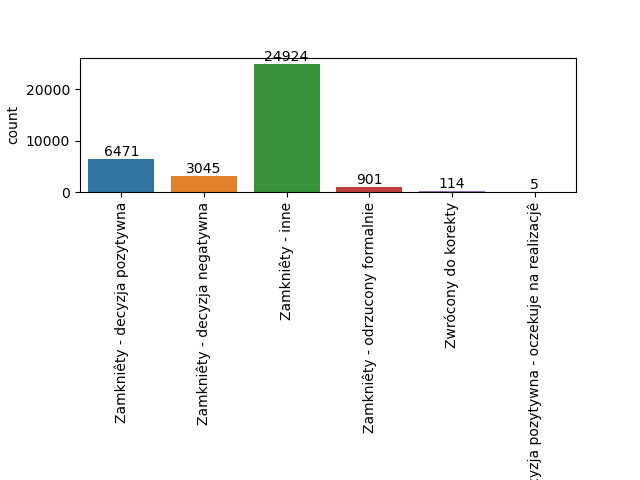
\includegraphics[width=0.5\textwidth]{img/application_status_countplot.png}
    \caption{Application status countplot}
    \label{fig:application_status_countplot}
\end{figure}

\begin{figure}
    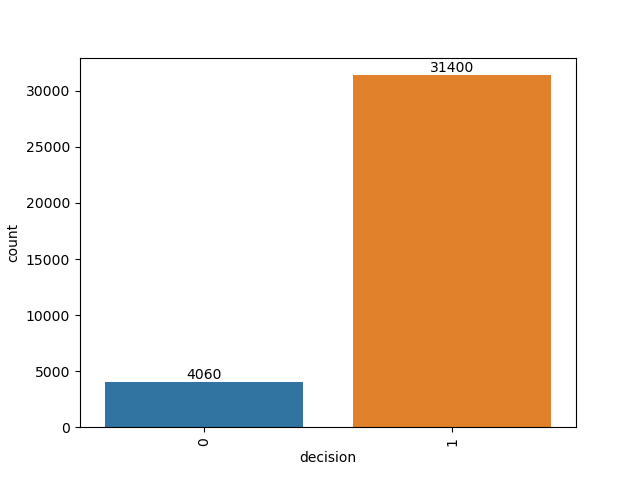
\includegraphics[width=0.5\textwidth]{img/decision_countplot.png}
    \caption{Decision countplot}
    \label{fig:decision_countplot}
\end{figure}

\begin{figure}
    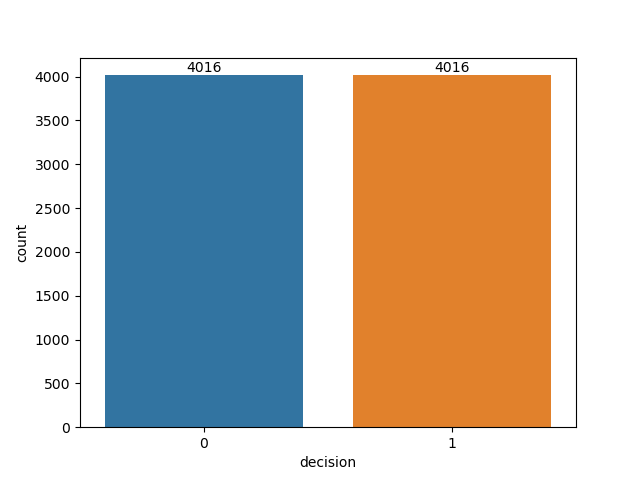
\includegraphics[width=0.5\textwidth]{img/balanced_decision_countplot.png}
    \caption{Balanced decision countplot}
    \label{fig:balanced_decision_countplot}
\end{figure}

\begin{table}
    \caption{Convert status into dean's decision.}
    \label{table:positive_negative}
    \begin{tabular}{|p{0.2\textwidth}|p{0.2\textwidth}|}
        \hline
            \textbf{positive} & \textbf{negative} \\
        \hline
            Zamkniety - decyzja pozytywna & Zamkniety - decyzja negatywna \\ 
        \hline
            Zamkniety - inne & Zamkniety - odrzucony formalnie \\
        \hline
            Decyzja pozytywna - oczekuje na realizacje & Zwrócony do korekty \\
        \hline
        
    \end{tabular}
    
\end{table}


\subsection{Data transformation}
At first columns which definitely should not be significant were removed. For example 'student' column was marked as not significant. The decision should not be performed according to ID of the person. All columns which should be significant was converted into numerical representation.
There was 42 columns in dataset. Only a few of them were numerical. Other were categorical. Using \textit{pd.factorize()} method unique values from each columns were extracted and converted into categorical codes.
There was two columns that were marked as significant, but were not converted into numberical representation due to complexity of the solutions. One of those was 'Level of thesis progress' which was not structured sentences with description about level of the thesis. The decision was made not to sink into this trying to convert it. The second column was 'Missing subjects codes' which had a form of `['A,B,C','C,D']` where letters were subject codes.


\section{Selecting features}

    % features selection description for the prediction problem (this is EDA) - here you should select most interesting features relevant for the specific type of application type using for the simplest case correlation coefficients
% EDA of selected features - here you should try to analyze the dependence of the features on the target value (the deans decision)

\begin{figure}
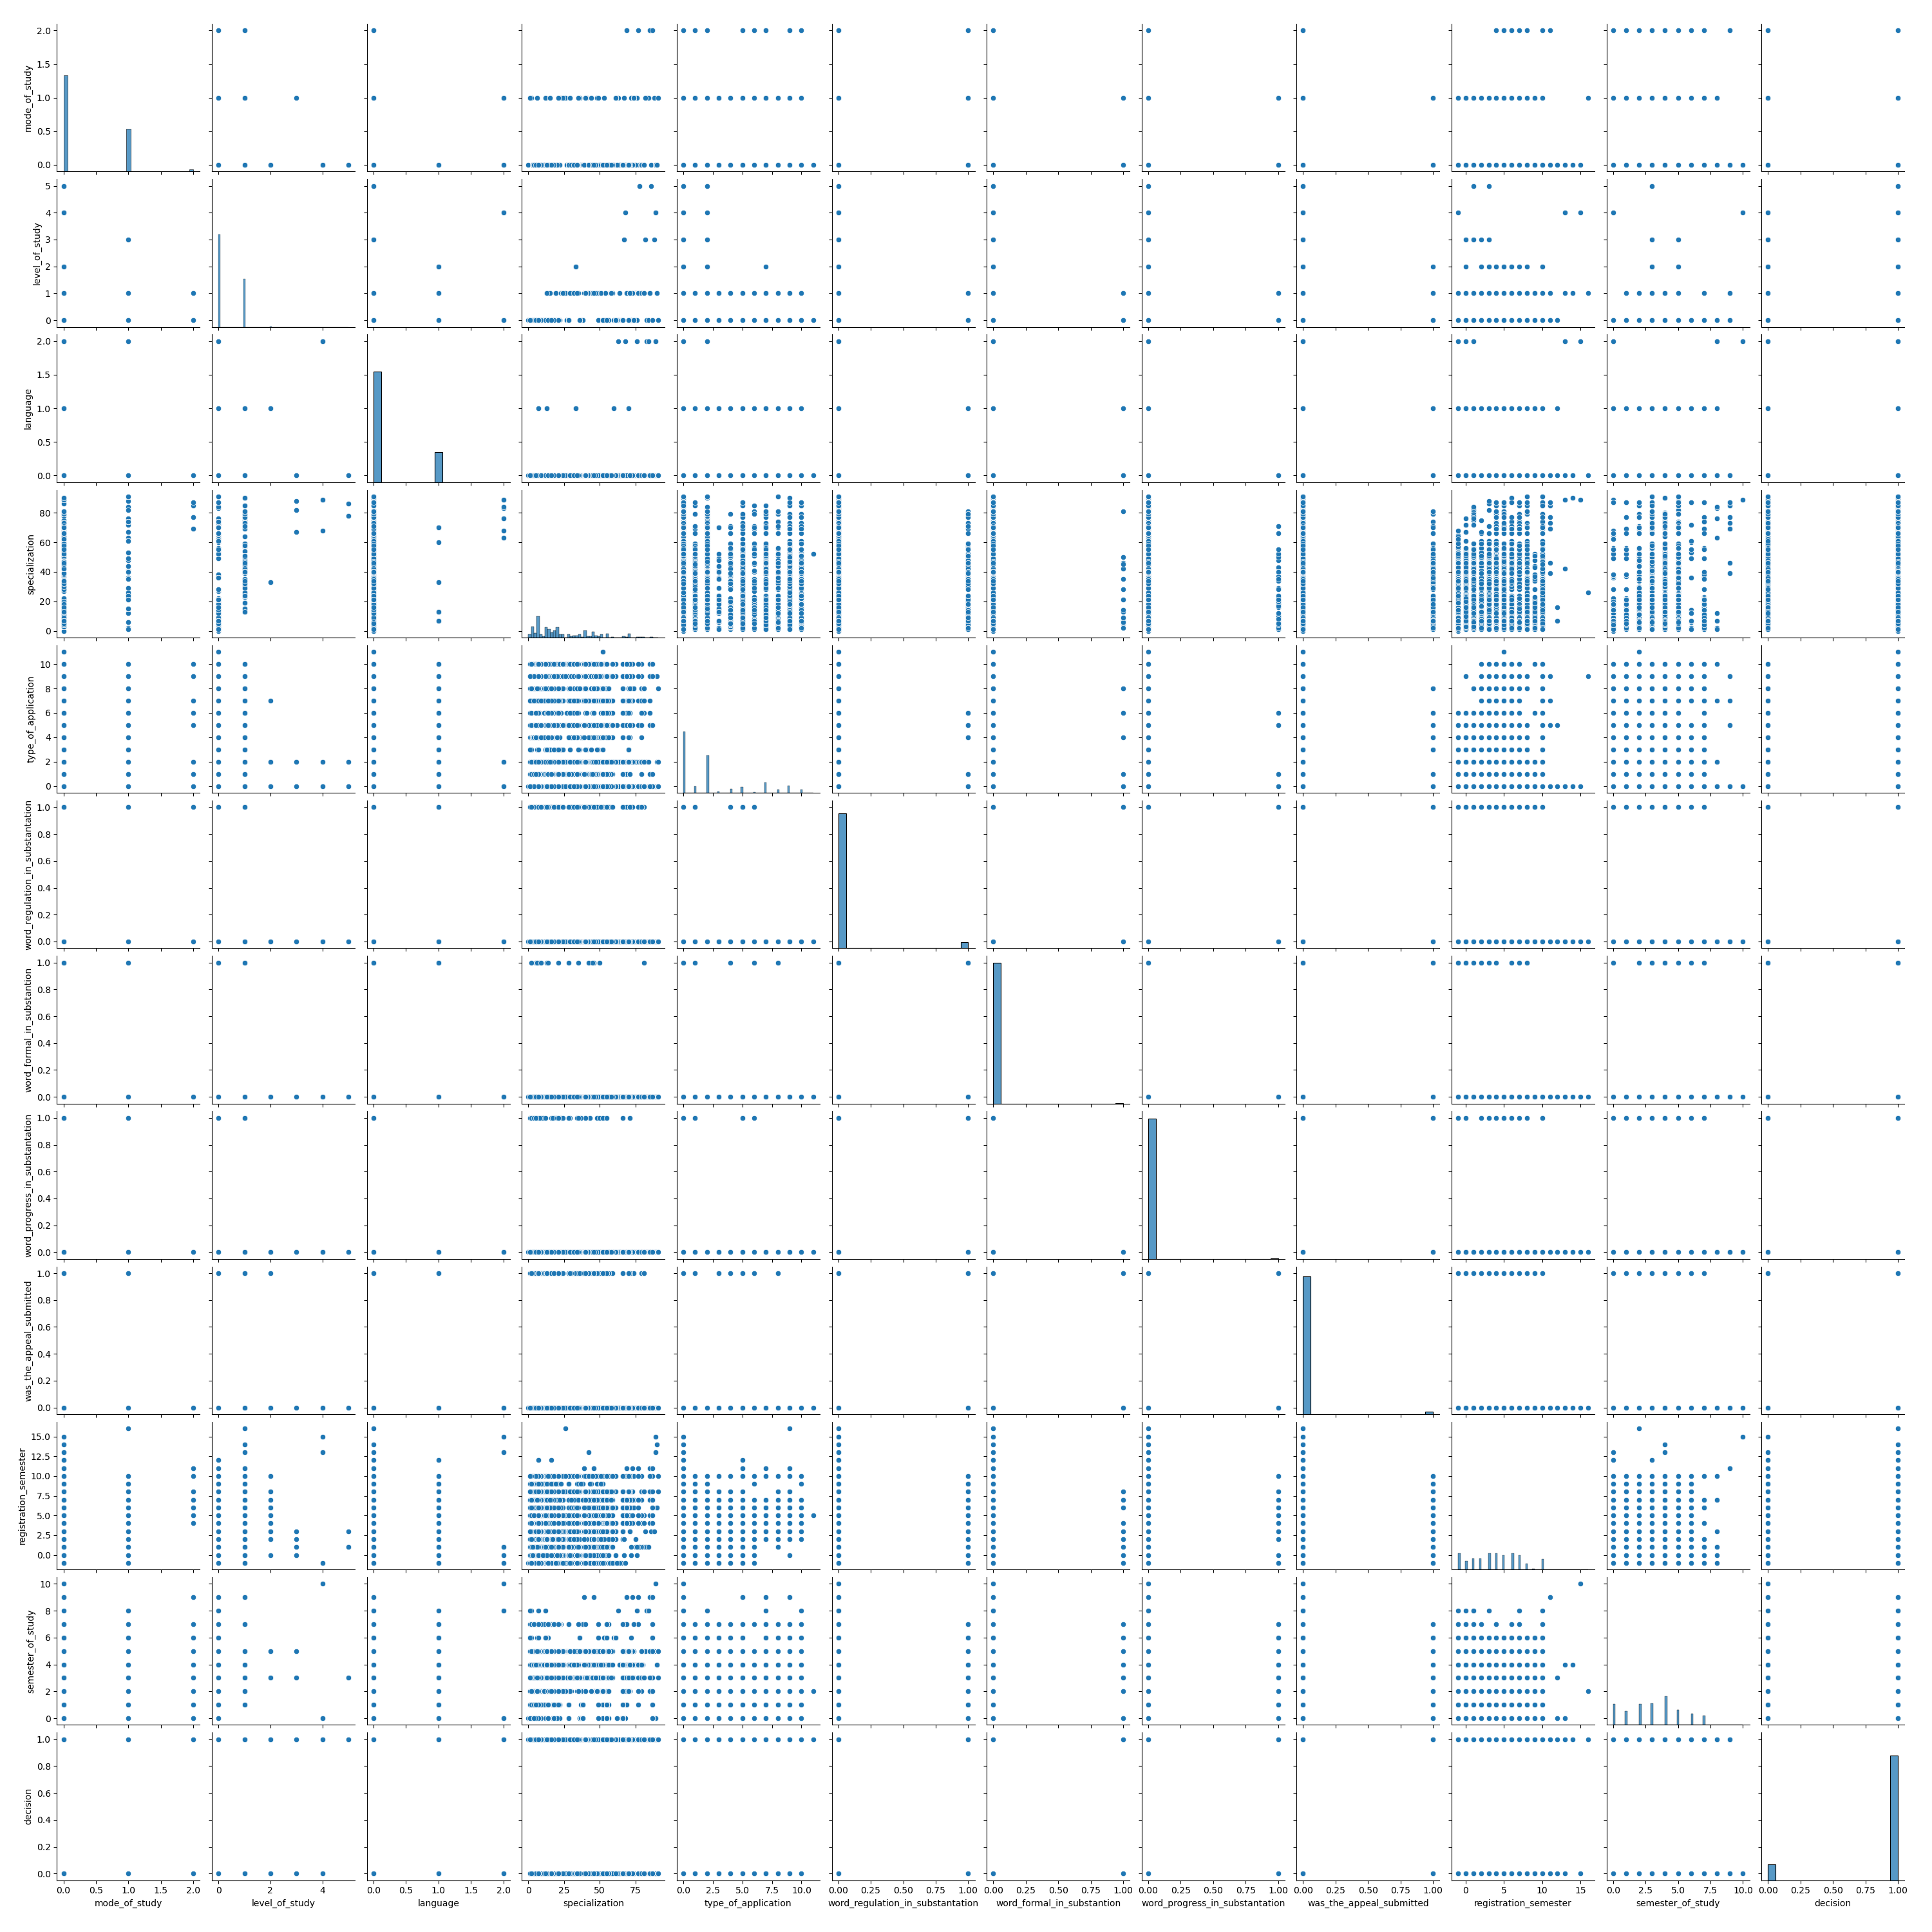
\includegraphics[width=0.5\textwidth]{img/pairplot.png}
\caption{Pairplot of all columns in dataset}
\label{fig}
\end{figure}

\section{Choosen algorithms}

    % selection and short theoretical description of two algorithms for the evaluation
% description of the benchmarking experiment - what are you going to check, verify and how you are going to get reasonable the results (eg. performance (classification metrics)),
According to sklearn library \cite{sklearn} and other\cite{towards_class} recomandation, the choosen was taken to train dataset with SVM model, Decision Tree Classifier and with KNN Classificator.

\subsection{SVM}

Support Vector Machine is a supervised machine learning algorithm used for classification and regression tasks. It finds an optimal hyperplane to separate data into different classes, using techniques like the kernel trick to handle non-linearly separable data\cite{tomaszkacmajor}. SVMs have advantages such as handling high-dimensional data and generalizing well with small datasets\cite{Zou}.

The basic idea behind SVM is to find an optimal hyperplane that separates the data points into different classes. A hyperplane is a decision boundary that divides the feature space into regions representing different classes. SVM aims to find the hyperplane that maximizes the margin, which is the distance between the hyperplane and the closest data points from each class. These closest data points are called support vectors\cite{PMC5822181}.

\subsection{Decision Tree Clasifier}

A Decision Tree Classifier is a machine learning algorithm that creates a tree-like model to classify data\cite{ibm_trees_decision_tree}. It recursively splits the dataset based on features, using decision rules to determine class labels. Decision trees are interpretable and easy to understand, but may overfit and perform poorly with high-dimensional or noisy data \cite{sklearn_tree}.

During the training phase, the decision tree classifier learns the decision rules by fitting the data to the tree structure \cite{Kotsiantis}. It continues splitting the data until a stopping criterion is met, such as reaching a maximum tree depth or when further splitting does not improve the classification accuracy. 

\subsection{KNN Classifier}

K-Nearest Neighbors Classifier is a simple and versatile algorithm for classification. It assigns a class label to a new data point based on the majority vote of its k nearest neighbors\cite{AbuAlfeilat}. KNN is easy to implement but can be computationally expensive for large datasets. It adapts well to different data types and handles multi-class classification\cite{Tsoumakas}.

KNN classifiers have several advantages, including their simplicity and ease of implementation. They can handle multi-class classification and can adapt to any kind of data. KNN is also a lazy learner, meaning it does not require an explicit training phase and can quickly adapt to new data. However, KNN can be computationally expensive, especially for large datasets, as it requires calculating distances for each prediction. Additionally, determining the optimal value of k and handling imbalanced data can be challenges in KNN classification\cite{Syaliman}.

\section{Evaluation}

    % tables with prediction results - showing that you have correctly applied the methods,
% tables evaluating performance (prediction metrics) for different types of application forms and both algorithms – this is the main part of the benchmark section,

\begin{figure}
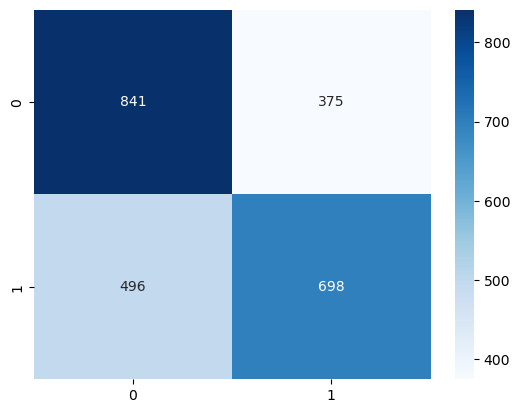
\includegraphics[width=0.5\textwidth]{img/svm_pred.png}
\caption{SVM model prediction}
\label{fig}
\end{figure}

\begin{figure}
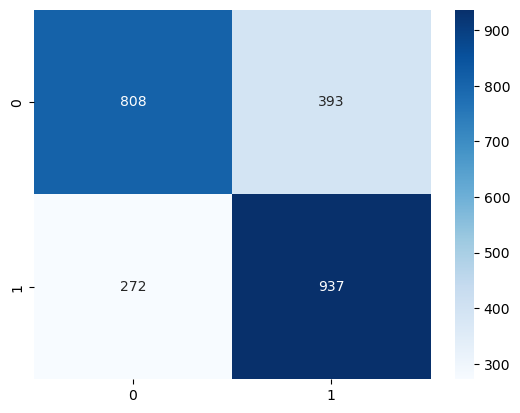
\includegraphics[width=0.5\textwidth]{img/dec_pred.png}
\caption{Decision Tree Classifier prediction}
\label{fig}
\end{figure}

\begin{figure}
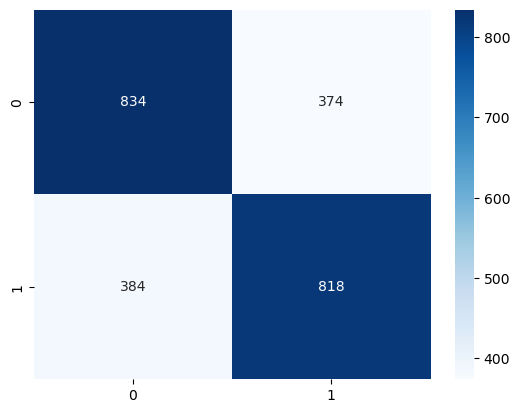
\includegraphics[width=0.5\textwidth]{img/knn_pred.png}
\caption{KNN Classifier prediction}
\label{fig}
\end{figure}

\begin{table}[htbp]
    \centering
    \caption{Comparison of ML Models}
    \label{tab:ml_comparison}
    \begin{tabular}{lccc}
        \hline
        \textbf{Model} & \textbf{Accuracy} & \textbf{Precision} & \textbf{Recall} \\
        \hline
        SVM & 0.64 & 0.64 & 0.64 \\
        Decision Tree Classifier & 0.72 & 0.73 & 0.73 \\
        KNN Classifier & 0.69 & 0.69 & 0.69 \\
        \hline
    \end{tabular}
\end{table}

\begin{table}[htbp]
    \centering
    \caption{Comparison of ML Models}
    \label{tab:ml_comparison}
    \begin{tabular}{lccc}
        \hline
        \textbf{Model} & \textbf{Accuracy} & \textbf{Precision} & \textbf{Recall} \\
        \hline
        SVM & 0.64 & 0.64 & 0.64 \\
        Decision Tree Classifier & 0.72 & 0.73 & 0.73 \\
        KNN Classifier & 0.69 & 0.69 & 0.69 \\
        \hline
    \end{tabular}
\end{table}

\section{Summary}

    % summary section (four to five sentences summing up the main outcomes of the paper - stress out the most important features, features which appeared to important by intuition but finally results in poor correlation, best performing algorithm,etc…)
The SVM model achieved an accuracy, precision, and recall of 0.64, indicating that it correctly predicts the class labels for 64\% of the data points. The Decision Tree Classifier performed slightly better, with an accuracy, precision, and recall of 0.68, correctly predicting the class labels for 68\% of the data points. The KNN Classifier showed similar performance, with an accuracy, precision, and recall of 0.69, correctly predicting the class labels for 69\% of the data points. These metrics provide insights into the models' ability to classify instances and predict positive class labels.

In summary, the KNN Classifier showed demonstrated the highest performance among the three models. These findings suggest that this classifierr may be the most effective choice for predicting the Dean's decision, considering its higher accuracy, precision and recall values.


\begin{thebibliography}{00}
% literature section should contain at least 4 to 5 positions from Google Scholar!
\bibitem{sklearn} https://scikit-learn.org/stable/tutorial/machine\_learning\_map/index.html
\bibitem{towards_class} https://towardsdatascience.com/top-10-binary-classification-algorithms-a-beginners-guide-feeacbd7a3e2
\bibitem{Zou} Zou, H. (2019). Classification with high dimensional features. Wiley Interdisciplinary Reviews: Computational Statistics, 11(1), e1453.
\bibitem{tomaszkacmajor} https://tomaszkacmajor.pl/index.php/2016/04/17/support-vector-machine/https://tomaszkacmajor.pl/index.php/2016/04/17/support-vector-machine/
\bibitem{PMC5822181} https://www.ncbi.nlm.nih.gov/pmc/articles/PMC5822181/
\bibitem{ibm_trees_decision_tree} https://www.ibm.com/docs/pl/spss-modeler/saas?topic=trees-decision-tree-models
\bibitem{sklearn_tree} https://scikit-learn.org/stable/modules/tree.html
\bibitem{Kotsiantis} Kotsiantis, S. B. (2013). Decision trees: a recent overview. Artificial Intelligence Review, 39(4), 261–283. https://doi.org/10.1007/s10462-011-9272-4
\bibitem{AbuAlfeilat} Abu Alfeilat, H. A., Hassanat, A. B. A., Lasassmeh, O., Tarawneh, A. S., Alhasanat, M. B., Eyal Salman, H. S., \& Prasath, V. B. S (2019). Effects of Distance Measure Choice on K-Nearest Neighbor Classifier Performance: A Review [Doi: 10.1089/big.2018.0175]. Big Data, 7(4), 221–248. https://doi.org/10.1089/big.2018.0175
\bibitem{Tsoumakas} Tsoumakas, G., Katakis, I., \& Vlahavas, I. (2006, September). A review of multi-label classification methods. In Proceedings of the 2nd ADBIS workshop on data mining and knowledge discovery (ADMKD 2006) (pp. 99-109).
\bibitem{Syaliman} Syaliman, K. U. (2021). Enhance the Accuracy of K-Nearest Neighbor (K-Nn) for Unbalanced Class Data Using Synthetic Minority Oversampling Technique (Smote) and Gain Ratio (Gr). INFOKUM, 10(1), 188-195.

\end{thebibliography}

\end{document}